\documentclass[cjk,slidestop,compress,mathserif,blue]{beamer}
%dvipdfm选项是关键,否则编译统统通不过
%beamer的颜色选项定义的是导航条和标题的颜色(即关键词structure的颜色)

%%%%%%%%%%%%%%%%仅限于XeTeX可使用的宏包%%%%%%%%%%%%%%%%%%%%%%%%%%%%
\usepackage{fontspec,xunicode,xltxtra,beamerthemesplit}
%\usepackage{beamerthemesplit}
\usepackage{xeCJK}
\setCJKmainfont[BoldFont=黑体, ItalicFont=楷体, BoldItalicFont=仿宋]{黑体}
%\setsansfont[Mapping=tex-text]{Adobe 黑体 Std}
%如果装了Adobe Acrobat,可在font.conf中配置Adobe字体的路径以使用其中文字体
%也可直接使用系统中的中文字体如SimSun,SimHei,微软雅黑 等
%原来beamer用的字体是sans family;注意Mapping的大小写,不能写错

%%%%%%%%   确定标题和导航条结构的框架     %%%%%%%%%%%%
\usepackage{beamerthemeshadow}                       %
%\usepackage{beamerthemeclassic}%导航条色与背景色一致%
%%%%%%%%%%%%%%%%%%%%%%%%%%%%%%%%%%%%%%%%%%%%%%%%%%%%%%
\setbeamerfont{roman title}{size={}}
%\usepackage{CJK} % CJK 中文支持                                  %
\usepackage{amsmath,amsthm,amsfonts,amssymb,bm}
\usepackage{mathrsfs}
\usepackage{xcolor}                                        %使用默认允许使用颜色
\usepackage{hyperref} 
\usepackage{graphicx}
\usepackage{subfigure}           %图片跨页

%\usepackage[numbers,sort&compress]{natbib} %紧密排列             %
\usepackage[sectionbib]{chapterbib}        %每章节单独参考文献   %
\usepackage{hypernat}                                                                         %
%\usepackage[dvipdfm,bookmarksopen=true,pdfstartview=FitH,CJKbookmarks]{hyperref}		%
\hypersetup{bookmarksnumbered,colorlinks,linkcolor=brown,citecolor=blue,urlcolor=red}         %
%参考文献含有超链接引用时需要下列宏包,注意与natbib有冲突        %
%\usepackage[dvipdfm]{hyperref}                                  %
%\usepackage{hypernat}                                           %
\newcommand{\upcite}[1]{\hspace{0ex}\textsuperscript{\cite{#1}}} %

%\useoutertheme{smoothbars}
\useinnertheme[shadow=true]{rounded}
\usetheme{Berkeley}                                          %主题式样
%\usetheme{Luebeck}

\usecolortheme{lily}                                        %颜色主题式样

\usefonttheme{professionalfonts}                           %字体主题样式宏包

%\beamertemplatetransparentcoveredhigh                      %使所有被隐藏的文本高度透明
\beamertemplatetransparentcovereddynamicmedium             %使所有被隐藏的文本完全透明,动态,动态的范围很小
\mode<presentation>
%\beamersetaveragebackground{gray}                          %设置背景颜色(单一色) 
\beamertemplateshadingbackground{green!10}{red!5}         %设置背景颜色(渐变色)

%在指定位置精确放置logo
\usepackage{tikz}
\usepackage{beamerfoils}
\usepackage{pgf}
\logo{\pgfputat{\pgfxy(11.68,0.15)}{
\includegraphics[height=1.01cm,viewport=0 0 140 120,clip]{Figures/BCC_logo-1.png}}\pgfputat{\pgfxy(10.502,-0.218)}{
\includegraphics[height=0.369cm,viewport=140 0 540 120,clip]{Figures/BCC_logo-1.png}}}
%\logo{\pgfputat{\pgfxy(11.68,0.15)}{
\includegraphics[height=0.95cm,viewport=0 0 510 360,clip]{Figures/Logo_Gainstrong.png}}\pgfputat{\pgfxy(10.333,-0.195)}{
\includegraphics[height=0.35cm,viewport=530 70 1100 218,clip]{Figures/Logo_Gainstrong.png}}}
%\MyLogo{
%	\pgfputat{\pgfxy(-50,-50)}{\pgfbox[right,base]{
\includegraphics[height=1cm]{Figures/BCC_logo-1.png}}}

%logo作为背景放置
%\setbeamertemplate{background}{
%	\pgfputat{\pgfxy(6.5,-0.5)}{\pgfbox[left,top]{\pgfimage[height=1.1cm]{Figures/BCC_logo-1.png}}}}

%\logo{}									%不显示logo

\begin{document}
%\begin{CJK*}{GBK}{song}
%\begin{CJK*}{GBK}{kai}
%beamer下不能用\songyi、\zihao等命令!
%\graphicspath{Figures/}

%-------------------------------PPT Title-------------------------------------
\title{APW-LAPW方法概述}
%-----------------------------------------------------------------------------

%----------------------------Author & Date------------------------------------
\author{北京市计算中心\;云平台\:姜骏}
\date{\textrm{2016.10.19}}
%\date{2013.09.10}
\frame{\titlepage}
%-----------------------------------------------------------------------------

%------------------------------------------------------------------------------列出全文 outline ---------------------------------------------------------------------------------
\section*{}
\frame[allowframebreaks]
{
  \frametitle{Outline}
%  \frametitle{\textcolor{mycolor}{\secname}}
  \tableofcontents%[current,currentsection,currentsubsection]
}
%在每个section之前列出全部Outline
%类似的在每个subsection之前列出全部Outline是\AtBeginSubsection[]
\AtBeginSection[]
{
  \frame<handout:0>
  {
    \frametitle{Outline}
%全部Outline中,本部分加亮
    \tableofcontents[current,currentsection]
  }
}

%------------------------------------------------------------------------------PPT main Body------------------------------------------------------------------------------------
\small
\section{APW方法}
\frame
{
	\frametitle{\textrm{Muffin-tin}近似}
\begin{figure}[h!]
\centering
\subfigure[\textrm{Muffin-tin Potentional}]{
\label{Semi-local-potential}
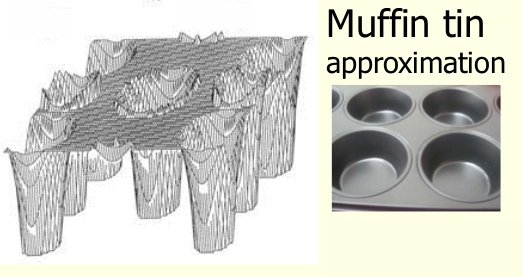
\includegraphics[height=1.10in,width=1.92in,viewport=1 22 507 295,clip]{Figures/Muffin-tin.png}}
\subfigure[\textrm{Division of the unit cell into spheres(I) and into interstitial region(II)}]{
\label{Semi-local-space}
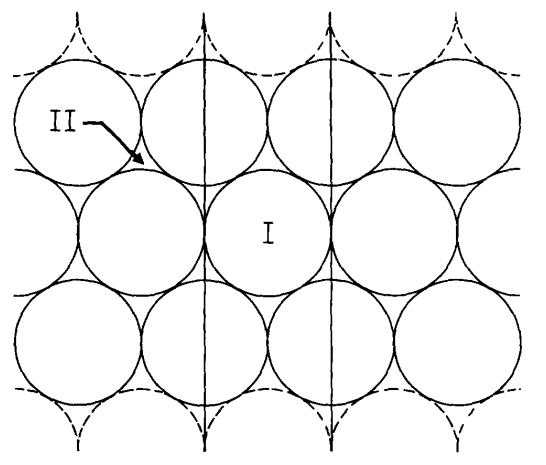
\includegraphics[height=1.45in,width=1.92in,viewport=1 20 515 435,clip]{Figures/Muffin-Tin.png}}
%\caption{\small \textrm{Division of the unit cell into spheres(I) and into interstitial region(II)}}%(与文献\cite{EPJB33-47_2003}图1对比)
\label{Muffin_tin-1}
\end{figure}
\textrm{Muffin-tin}近似是\textrm{Johnson}采用$\chi_{\alpha}$方法计算分子体系的交换-相关时,引入多重散射(\textrm{Multiple scattering})理论时提出的%,\textrm{Muffin-tin}直译为“松饼罐头”,意思是把分子中的原子看成堆在一起的圆球罐

\textcolor{red}{\textrm{MT}球近似与多重散射理论有密切的关联}
}

\frame
{
\frametitle{\textrm{APW}方法}
\begin{figure}[h!]
\centering
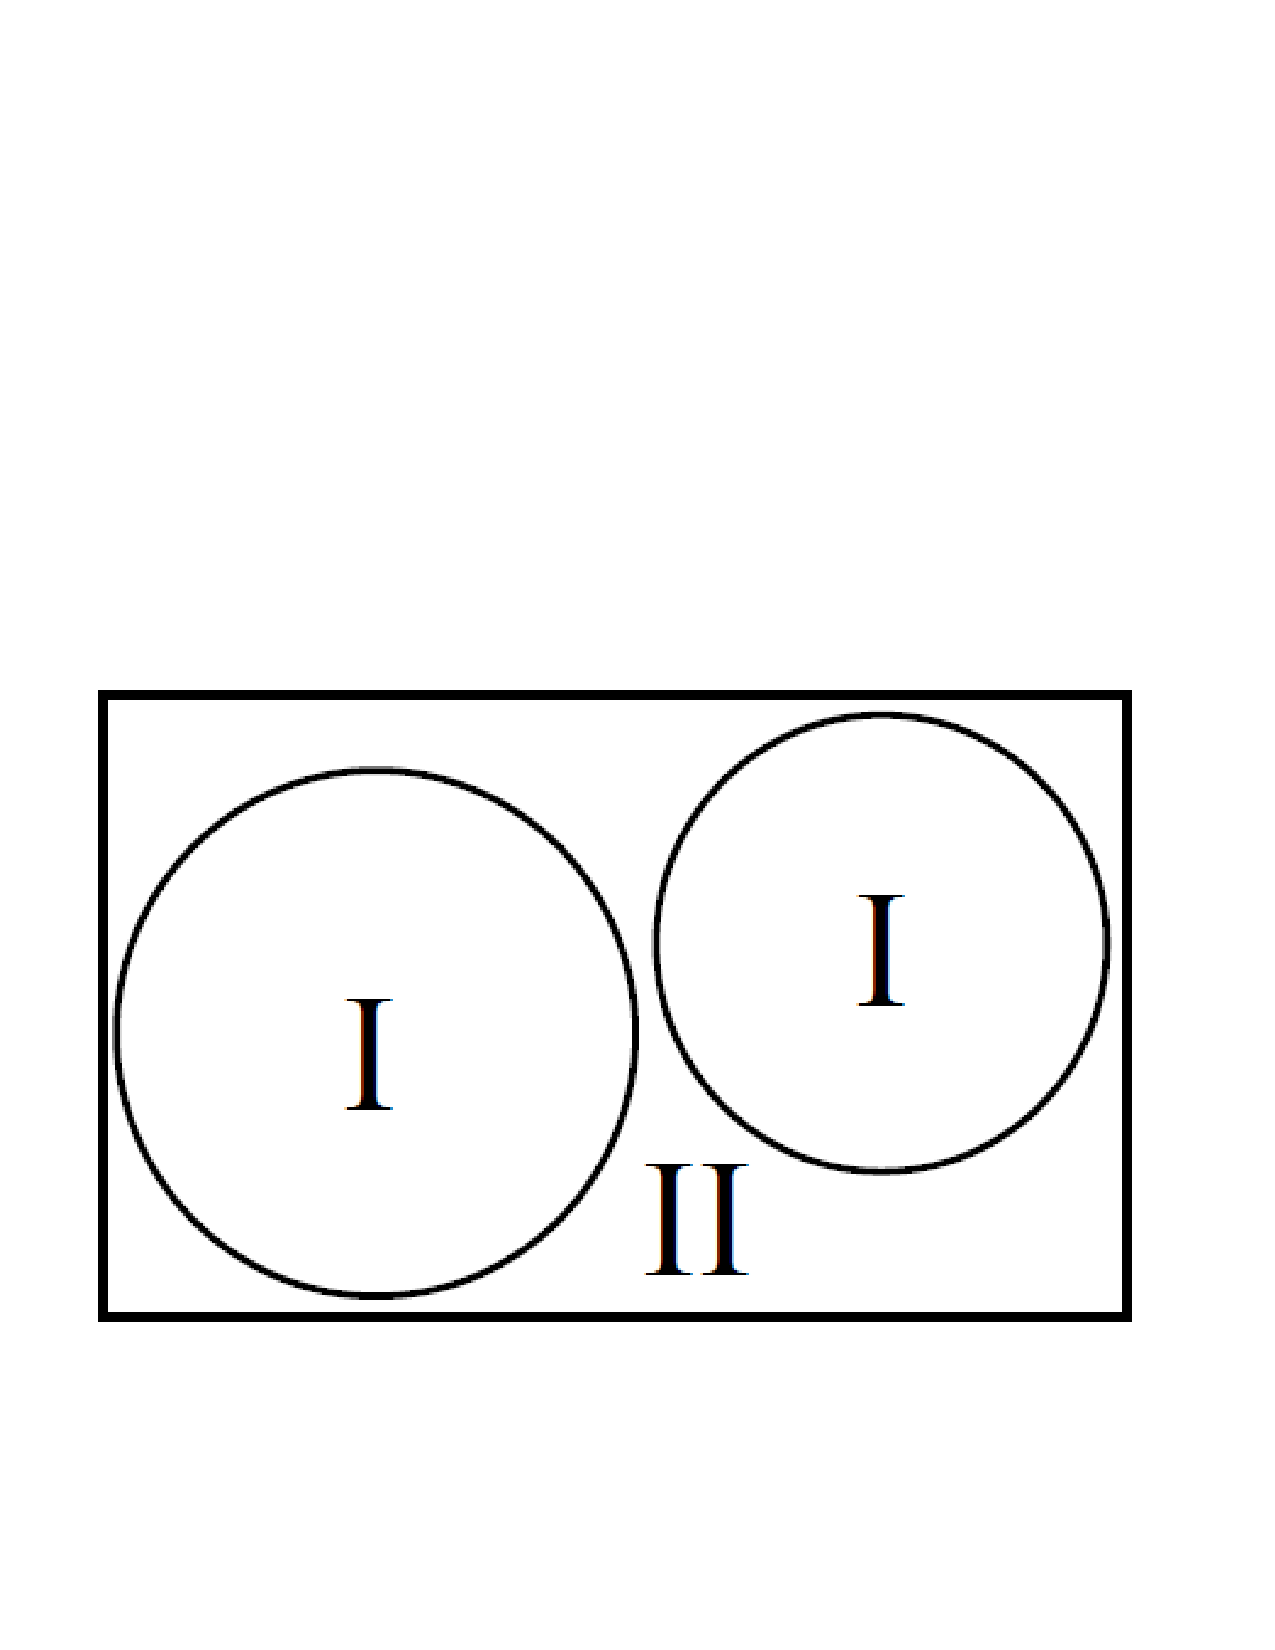
\includegraphics[height=1.10in,width=1.80in,viewport=40 150 545 465,clip]{Figures/Muffin_tin.pdf}
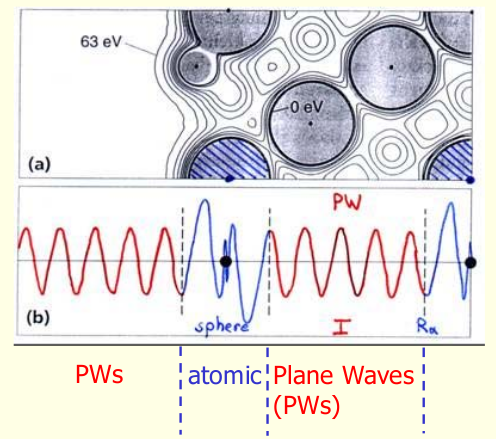
\includegraphics[height=1.10in,width=1.45in,viewport=1 20 485 435,clip]{Figures/APW.png}
\caption{\small \textrm{Partitioning of the unit cell into atomic spheres(I) and an interstitial region(II)}}%(与文献\cite{EPJB33-47_2003}图1对比)
\label{Muffin_tin-2}
\end{figure}
\begin{displaymath}
\hskip -28pt\footnotesize \varphi(\vec k_j,\vec r)=\left\{
  \begin{aligned}
	  &\Omega^{-1/2}\mathrm{e}^{\mathrm{i}\vec k_j\cdot\vec r_s}\mathrm{e}^{\mathrm{i}\vec k_j\cdot(\vec r-\vec r_s)},&|\vec r-\vec r_s|>R_{\mathrm{MT}}^s\\
	  &\sum_{lm}A_{lm}^{\vec k_j}u_l(|\vec r-\vec r_s|,E)Y_{lm}(\widehat{\vec r-\vec r_s}),&|\vec r-\vec r_s|\leqslant R_{\mathrm{MT}}^s
  \end{aligned}
\right.
\end{displaymath}
}

\frame
{
	\frametitle{空间两部分函数在球面上的衔接}
	根据\textrm{Huygens}原理:\textcolor{blue}{平面波可以在各个原子球中心用球面波展开}:
	\begin{displaymath}
		\mathrm{e}^{\mathrm{i}\vec k\cdot\vec r}=4\pi\sum_{l=0}^{\infty}\sum_{m=-l}^l\mathrm{i}^lj_l(|\vec k|r)Y_{lm}^{\ast}(\hat{\vec k})Y_{lm}(\hat{\vec r})
	\end{displaymath}
	其中$j_l(|\vec k|r)$是$l$-阶球\textrm{Bessel}函数,$\hat{\vec k}$和$\hat{\vec r}$分别是矢量$\vec k$和$\vec r$与直角坐标$z$-轴的夹角$\theta$和$\varphi$

	要求空间中不同区域函数在球面上连续,可调参数$A_{lm}^{\vec k}$可为下式确定
\begin{displaymath}
	A_{lm}^{\vec k}=4\pi\mathrm{e}^{\mathrm{i}\vec k\cdot\vec r_s}\mathrm{i}^lY_{lm}^{\ast}(\hat{\vec k})j_l(|\vec k|R_{MT}^s)/u_l(R_{MT}^s,E)
\end{displaymath}
\textrm{APW}的问题:\textcolor{blue}{球面参数$A_{lm}^{\vec k}$对能量$E$依赖,由此构造的久期方程是非线性的}
}

\section{LAPW方法}
\frame
{
\frametitle{\textrm{LAPW}方法}
%\small\textrm{APW}方法的困难,久期方程不能化成广义本征值方程的形式(久期方程对能量$E$是非线性的)为了克服这一困难,人们提出线性化方法,
\textrm{O.~K.~Andersen~}提出\textrm{LAPW}方法\upcite{Singh_Book}:将$u_l(r,E)$在某一合适的$E_l$值附近对$E$的一阶微商{\footnotesize$\left.\dfrac{\textrm{d}u_l(r,E)}{\textrm{d}E}\right|_{E_l}\equiv\dot u_l(r,E_l)$}\\代入\textrm{APW}基函数中可得\textrm{LAPW}方法的基函数:
$${\footnotesize\hskip -50pt \varphi(\vec k_j,\vec r)=\left\{
  \begin{aligned}
    &\Omega^{-1/2}\exp[i\vec k_j\cdot\vec r],&|\vec r-\vec r_s|>R_{\mathrm{MT}}^s\\
    &\sum_{lm}[A^{\vec k_j}_{lm}u_l(|\vec r-\vec r_s|,E_l)+B^{\vec k_j}_{lm}\dot u_l(|\vec r-\vec r_s|,E_l)]Y_{lm}(\widehat{\vec r-\vec r_s}),&|\vec r-\vec r_s|\leqslant R_{\mathrm{MT}}^s
  \end{aligned}
\right.}$$
%$$\Psi_{\vec k}(\vec r)=\int_{\Omega}\tilde G_{\vec k}(\vec r-\vec r\,^\prime;E)V(\vec r\,^\prime)\Psi_{\vec k}(\vec r\,^\prime)\textrm{d}\vec r\,^\prime$$
根据基函数在\textrm{MT}球面上连续到一阶,确定系数$A^{\vec k}_{lm}$,$B^{\vec k}_{lm}$的值。
\begin{figure}[h!]
\centering
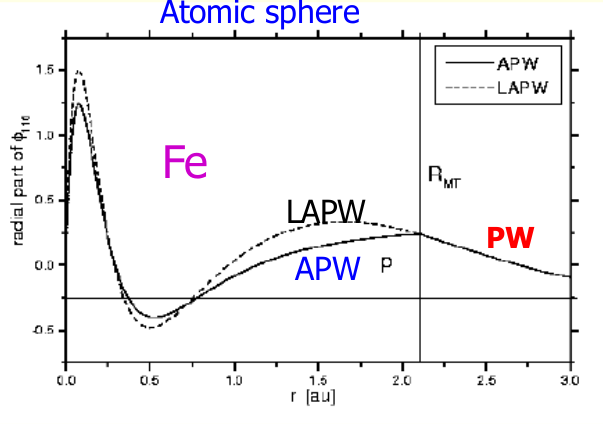
\includegraphics[height=1.20in,width=1.98in,viewport=1 20 585 435,clip]{Figures/WIEN2k-LAPW.png}
\caption{\small \textrm{Partitioning of the unit cell into atomic spheres(I) and an interstitial region(II)}}%(与文献\cite{EPJB33-47_2003}图1对比)
\label{Muffin_tin}
\end{figure}
}

\frame
{
	\frametitle{\textrm{semi-core}与\textrm{Ghost-band}}
\begin{figure}[h!]
\centering
\vspace*{-0.2in}
\hspace*{-0.2in}
\subfigure[\textrm{Windows with a semi-core state}]{
\label{Semi-local-1}
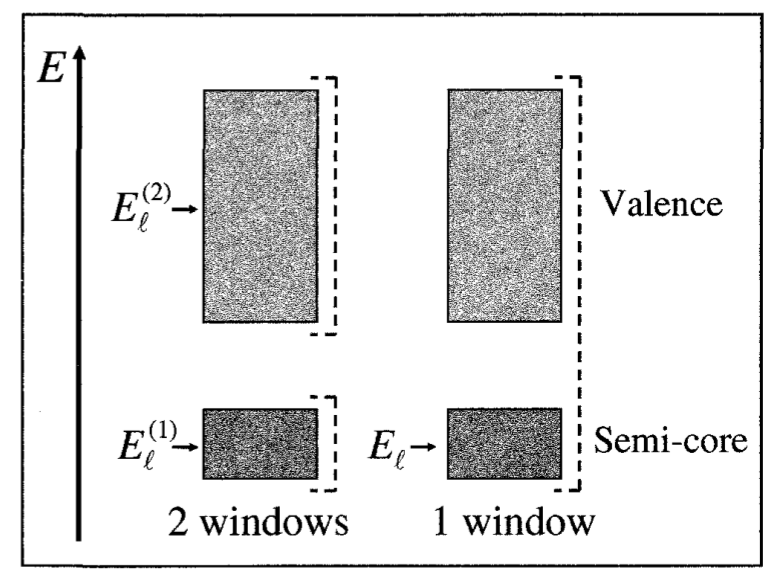
\includegraphics[height=1.88in,width=2.35in,viewport=0 0 785 615,clip]{Figures/Ghost-Multi_Windows.png}}
\subfigure[\textrm{Variation of a semi-core and a valence band with $E_l$}]{
\label{Semi-local-2}
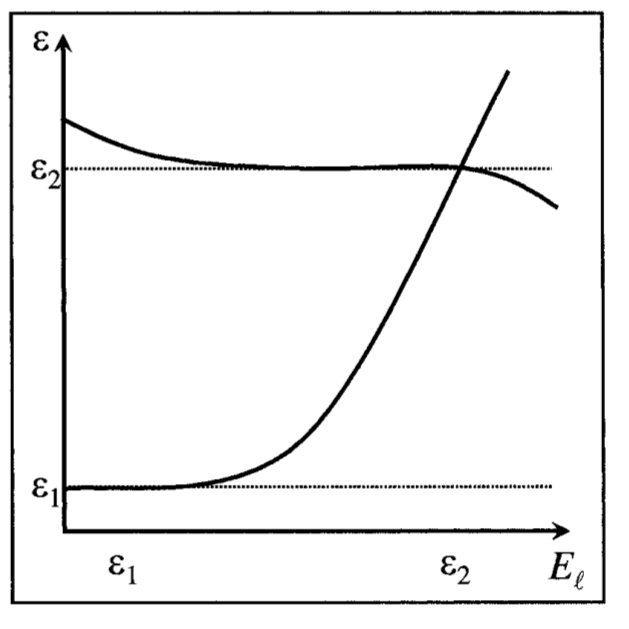
\includegraphics[height=1.88in,width=1.54in,viewport=0 0 625 650,clip]{Figures/Ghost-Multi_energy.png}}
\label{Semi-local}
\end{figure}
}

\frame
{
\frametitle{\textrm{LO}基函数}
为提高\textrm{LAPW}方法的变分自由度,在同一能量范围处理半芯态(接近价态的能量较高的芯态)和价态,可添加与$\vec k$无关的基函数,称为局域轨道(\textrm{local orbitals, LO})%。据此构造的基函数称为%包含两个指定能量的径向波函数和其中一个能量导数,这样的基函数即LAPW+
或\textrm{LO}基函数:
{\footnotesize
$$\hskip -22pt \phi_{lm}^{\mathrm{LO}}(\vec r)=\left\{
  \begin{aligned}
    &[A_{lm}u_l(r,E_{1,l})+B_{lm}\dot u_l(r,E_{1,l})+C_{lm}u_l(r,E_{2,l})]Y_{lm}(\hat{\vec r})\quad&r\leqslant R_{\mathrm{MT}}^s\\
    &0 &r>R_{\mathrm{MT}}^s
\end{aligned}
\right.$$}

类似地,根据$\phi_{lm}^{\mathrm{LO}}(\vec r)$在\textrm{MT}球面上的数值为零、一阶导数为零,并且$\phi_{lm}^{\mathrm{LO}}(\vec r)$在\textrm{MT}球内归一化的要求,可以确定系数$A_{lm}$,$B_{lm}$,$C_{lm}$的值。
\begin{figure}[h!]
	\vspace{-15pt}
\centering
\hspace{15pt}
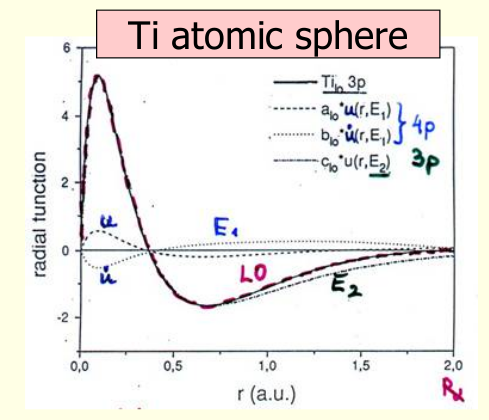
\includegraphics[height=1.45in,width=1.55in,viewport=50 10 470 415,clip]{Figures/WIEN2k-lo.png}
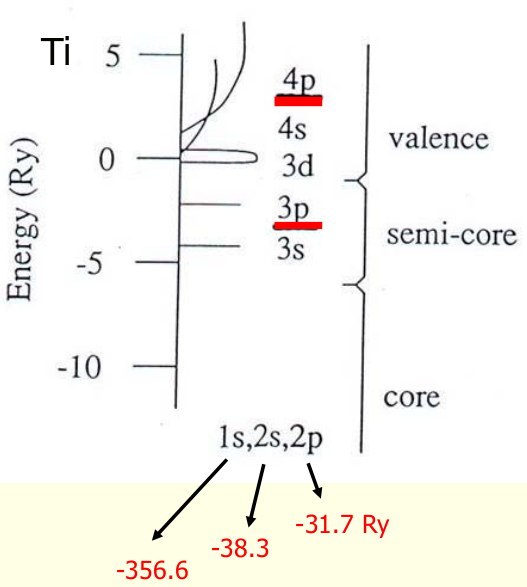
\includegraphics[height=1.45in,width=1.45in,viewport=5 1 570 570,clip]{Figures/semi-core.png}
\caption{\small \textrm{}}%(与文献\cite{EPJB33-47_2003}图1对比)
\label{Muffin_tin_LO}
\end{figure}
}

\frame
{
\frametitle{\textrm{APW+lo}基函数}
\textrm{Sj\"ostedt}等发现上述\textrm{LAPW}方法并非是\textrm{APW}方法线性化的最有效方法。采用指定能量参数$E_l$的\textrm{APW}形式的径向波函数,外加\textrm{APW}型局域轨道(\textrm{local orbit, lo})基函数,是更有效的方案,称为\textrm{APW+lo}方法\upcite{SSC114-15_2000}。
$$  \varphi(\vec k_j,\vec r)=\left\{
  \begin{aligned}
    &\sum_{lm}[A^{\vec k_j}_{lm}u_l(r,E_l)]Y_{lm}(\hat{\vec r})\quad&r\leqslant R_{\mathrm{MT}}^s\\
    &\Omega^{-1/2}\exp(i\vec k_j\cdot\vec r) &r>R_{\mathrm{MT}}^s
  \end{aligned}\right.
  \label{eq:APW-basis}
$$
$$  \phi_{lm}^{\mathrm{lo}}(\vec r)=\left\{
  \begin{aligned}
  &[A_{lm}u_l(r,E_{1,l})+B_{lm}\dot u_l(r,E_{1,l})]Y_{lm}(\hat{\vec r})\quad&r\leqslant R_{\mathrm{MT}}^s\\
  &0&r>R_{\mathrm{MT}}^s
  \end{aligned}
\right.$$
\textrm{APW+lo}基函数式形式上与标准\textrm{LAPW}基函数式形式非常相似,但\textrm{APW+lo}基函数是平滑且一阶可微的,在\textrm{MT}球面上有动能对\textrm{Hamiltonian}的贡献需要计算。计算表明,采用\textrm{APW+lo}基组比标准\textrm{LAPW}基组计算效率高。
}

\frame
{
\frametitle{\textrm{WIEN2k}程序中基函数的选择}
\begin{figure}[h!]
	\vspace{-15pt}
\centering
\hspace{15pt}
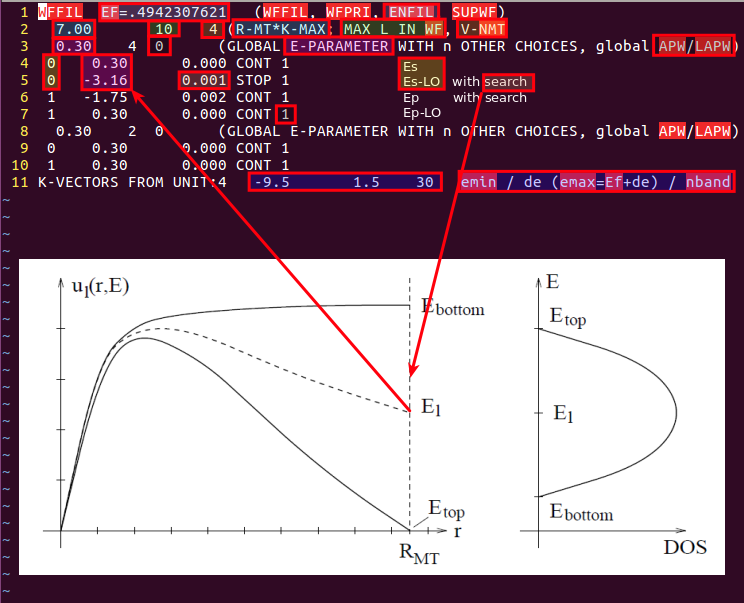
\includegraphics[height=2.55in,width=3.35in,viewport=10 30 750 605,clip]{Figures/WIEN2k-in1.png}
\caption{\small \textrm{The parameter $\mathrm{E}_l$ in case.in1 for WIEN2k.}}%(与文献\cite{EPJB33-47_2003}图1对比)
\label{WIEN2k-in1}
\end{figure}
}

\frame
{
	\frametitle{固体计算方法总结}
\begin{figure}[h!]
\centering
\vspace*{-0.25in}
%\hspace*{-0.80in}
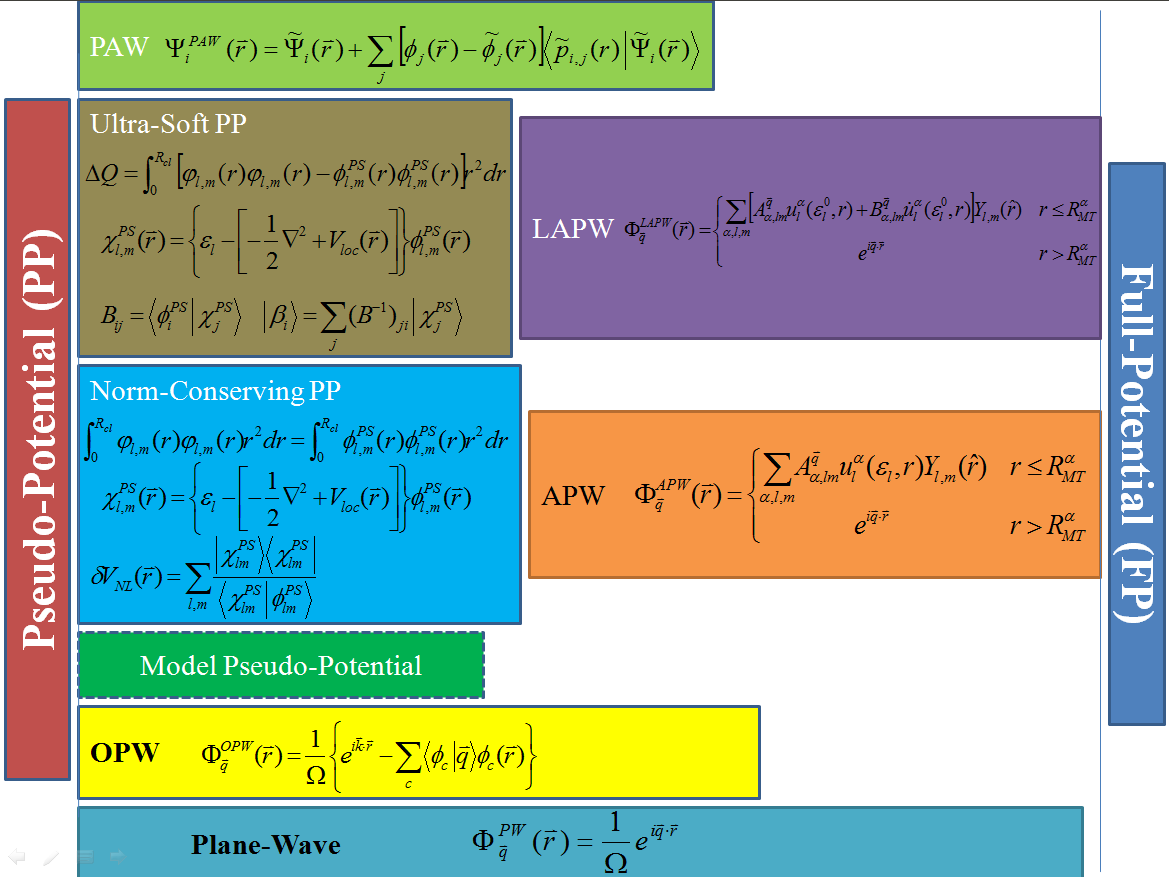
\includegraphics[height=2.80in,width=4.10in,viewport=0 0 1190 876,clip]{Figures/Pseudo-Full_Potential.png}
%\caption{\small \textrm{Pseudopotential for metallic sodium, based on the empty core model and screened by the Thomas-Fermi dielectric function.}}%(与文献\cite{EPJB33-47_2003}图1对比)
\label{Pseudo-Full_Poential}
\end{figure}
}

%\frame
%{
%\frametitle{发展统一理论框架下的材料计算程序}
%\begin{itemize}
%	\item
%\end{itemize}
%}

\appendix
%------------------------------------------------------------------------Reference----------------------------------------------------------------------------------------------
%\begin{thebibliography}{99}
%-----------------------------------------------------------------------------------------------------------------------------------------------------------------------%
%\frame
%{
%\frametitle{主要参考文献}
%{\small
%\bibitem{Singh_Book}\textrm{D. J. Singh. \textit{Plane Wave, PseudoPotential and the LAPW method} (Kluwer Academic, Boston,USA, 1994)}					%
%  \nocite{*}																				%
%}
%}
%\end{thebibliography}
\begin{thebibliography}{99}
\frame
{
\frametitle{主要参考文献}
{\small
%	\bibitem{Huang_Han}黄昆\:原著、韩汝琦\:改编, {\textit{固体物理学}}\:高等教育出版社, 北京, 1988
%	\bibitem{Xie_Lu}谢希德、陆栋\:主编, {\textit{固体能带理论}}\:复旦大学出版社, 上海, 1998
        \bibitem{Singh_Book}\textrm{D. J. Singh. \textit{Plane Wave, PseudoPotential and the LAPW method} (Kluwer Academic, Boston,USA, 1994)}
	\bibitem{Comp_Method}\textrm{V. V. Nemoshkalenko and V. N. Antonov. \textit{Computational Methods in Solid State Physics} (Gordon and Breach Science Publisher, Amsterdam, The Netherlands, 1998)}
	\bibitem{JMP22-2433_1981}\textrm{M. Weiner. \textit{J. Math. Phys.}, \textbf{22} (1981), 2433}
%	\bibitem{PRB26-4571_1982}\textrm{M. Weinert, E. Wimmer and A. J. Freeman. \textit{Phys. Rev.} B, \textbf{26} (1982), 4571}
	\bibitem{SSC114-15_2000}\textrm{E. Sj\"ostedt, L. Nordstr\"om and D. J. Singh. \textit{Solid State Commun.}, \textbf{114} (2000), 15}
	\bibitem{Elect_Stru}\textrm{Richard. M. Martin. \textit{Electronic Structure: Basic Theory and Practical Methods} (Cambridge University Press, Cambridge, England, 2004)}
}
\nocite*{}
}
\end{thebibliography}
%{\small
%\phantomsection\addcontentsline{toc}{section}{Bibliography}	 %直接调用\addcontentsline命令可能导致超链指向不准确,一般需要在之前调用一次\phantomsection命令加以修正	%
%\bibliography{Myref}																			%
%\bibliographystyle{mybib}																		%
%  \nocite{*}																				%
%}
%-----------------------------------------------------------------------------------------------------------------------------------------------------------------------%


%-----------------------------------------------------------Beamer下不建议使用bib,因为涉及分页--------------------------------------------------------------------------%
%{\small
%\phantomsection\addcontentsline{toc}{section}{Bibliography}	 %直接调用\addcontentsline命令可能导致超链指向不准确,一般需要在之前调用一次\phantomsection命令加以修正	%
%\bibliography{Myref}																			%
%\bibliographystyle{mybib}																		%
%  \nocite{*}																				%
%}

%------------------------------------------------------------------------------------------------------------------------------------------------------------------------------%

%-------------------------------------------------------------------------Thanks------------------------------------------------------------------------------------------------
%\section{致谢}
%\frame
%{
%\frametitle{致$\quad$谢}
%\begin{itemize}
%    \setlength{\itemsep}{20pt}
%  \item 感谢本团队高兴誉、吴泉生、宋红州等各位老师参与的讨论
%  \item 感谢莫所长、宋主任以及软件中心各位老师和同事
%  \item 感谢王崇愚先生的帮助
%\end{itemize}
%}

\logo{}									%不显示logo
\frame
{
\vskip 60 pt
%\hskip 10pt \textcolor{blue}{\Huge 感谢答辩委员会各位老师\,\textrm{!}}\\
\vskip 35 pt
\hskip 60pt \textcolor{blue}{\Huge 谢谢大家\:!}
%\vskip 15 pt
%\hskip 40pt \textcolor{blue}{\Huge \textrm{for your attention\:!}}
}

%-------------------------------------------------------------------------------------------------------------------------------------------------------------------------------

\clearpage
%\end{CJK*}
\end{document}
